%Beamer class
\documentclass{beamer}

\usepackage[czech]{babel}
\usepackage[cp1250]{inputenc}
\usepackage{fontenc}
\usepackage{tgheros}
\usepackage{array}
\usepackage{color}
\usepackage{hyperref}

\usetheme{Antibes}
\usecolortheme{crane}


\title[BE1M13VES]{BE1M13VES}
\subtitle[Manufacturing of Electrical Components] {Manufacturing of Electrical Components}
\author[Brejcha]{Michal Brejcha}
\institute[CTU]{CTU in Prague}
\date[Prague, 2017]{Prague, 2017}

\begin{document}
%------------------------------------------------------------------------------
%Uvodni slajd
%------------------------------------------------------------------------------
\frame{\titlepage}

\begin{frame}
\frametitle{Overview} 
\tableofcontents
\end{frame}

\AtBeginSection[]
{
  \begin{frame}
    \frametitle{TOPIC}
    \tableofcontents[currentsection]
  \end{frame}
}

%------------------------------------------------------------------------------
%Photodiodes and LEDs
%------------------------------------------------------------------------------
\section{\texorpdfstring{Photodiodes and LEDs}{Photodiodes and LEDs}}
%------------------------------------------------------------------------------
	\begin{frame}
    \frametitle{Photoelectric effect}
		\begin{center}
			\begin{tabular}{m{0.4\linewidth} m{0.5\linewidth}}
			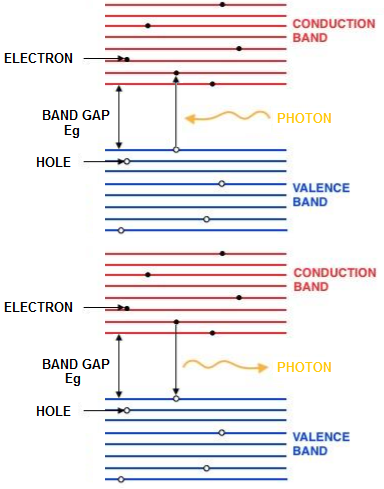
\includegraphics[scale=0.43]{obr10_fotoel.png} &
			\small
			\begin{itemize}
				\item Each photon carries particular amount of energy.
				\item Collision with electron may push the electron to higher energy state.
				\item The energy of the photon must be: $E \geq h\cdot f$
				
				\begin{itemize}
					\item[h]... Planck constant
					\item[f]... photon frequency
				\end{itemize}
				\item Rest of the energy is converted to heat.
			\end{itemize}
			\end{tabular}
		\end{center}
	\end{frame}
%------------------------------------------------------------------------------
	\begin{frame}
    \frametitle{Photoelectric effect}
		\begin{center}
			\begin{tabular}{m{0.4\linewidth} m{0.5\linewidth}}
			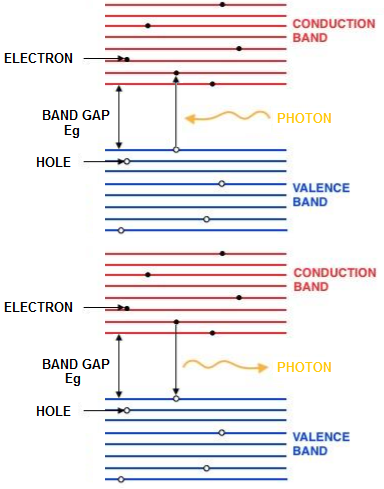
\includegraphics[scale=0.43]{obr10_fotoel.png} &
			\small
			\begin{itemize}
				\item The energy is released as photon during recombination.
				\item The photon wavelength $\lambda$ is given by the band gap: $$f=\frac{E_g}{h}=\frac{c}{\lambda}$$
				
				\begin{itemize}
					\item[c]... speed of the light
				\end{itemize}
				\item Recombination process is used in LEDs.
			\end{itemize}
			\end{tabular}
		\end{center}
	\end{frame}
%------------------------------------------------------------------------------
	\begin{frame}
    \frametitle{Light Emitting Diode}
			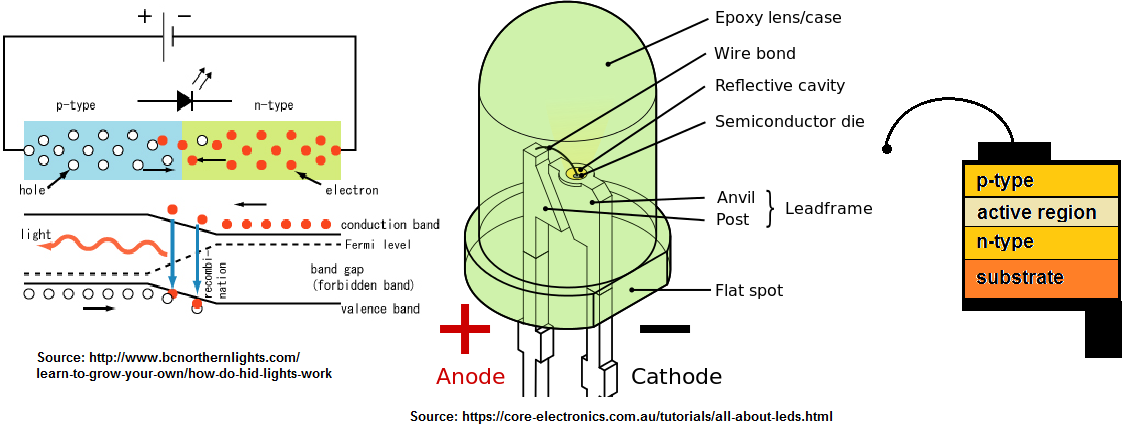
\includegraphics[scale=0.35]{obr11_LED.png}
		\small
		\begin{itemize}
			\item Color depends on the bandgap: \\InGaN (blue, UV, green), AlGaInP (yellow, orange), AlGaAs (red, IR), GaP (yellow, green)
			\item Similar characteristic to ordinary diode - higher threshold voltages (\textcolor{red}{IR 1,2 V}; \textcolor{red}{RED 1,8 V}; \textcolor{orange}{YELLOW 2,2 V}; \textcolor{blue}{BLUE 3,6 V}).
		\end{itemize}
	\end{frame}
%------------------------------------------------------------------------------
	\begin{frame}
    \frametitle{Photodiode}
		The PN junction is accessible to light via anti-reflection layer. The light creates other pairs of electron and holes, that are swept by the electric field of depletion area to the \textbf{n} (electrons) and \textbf{p} (holes) part.
		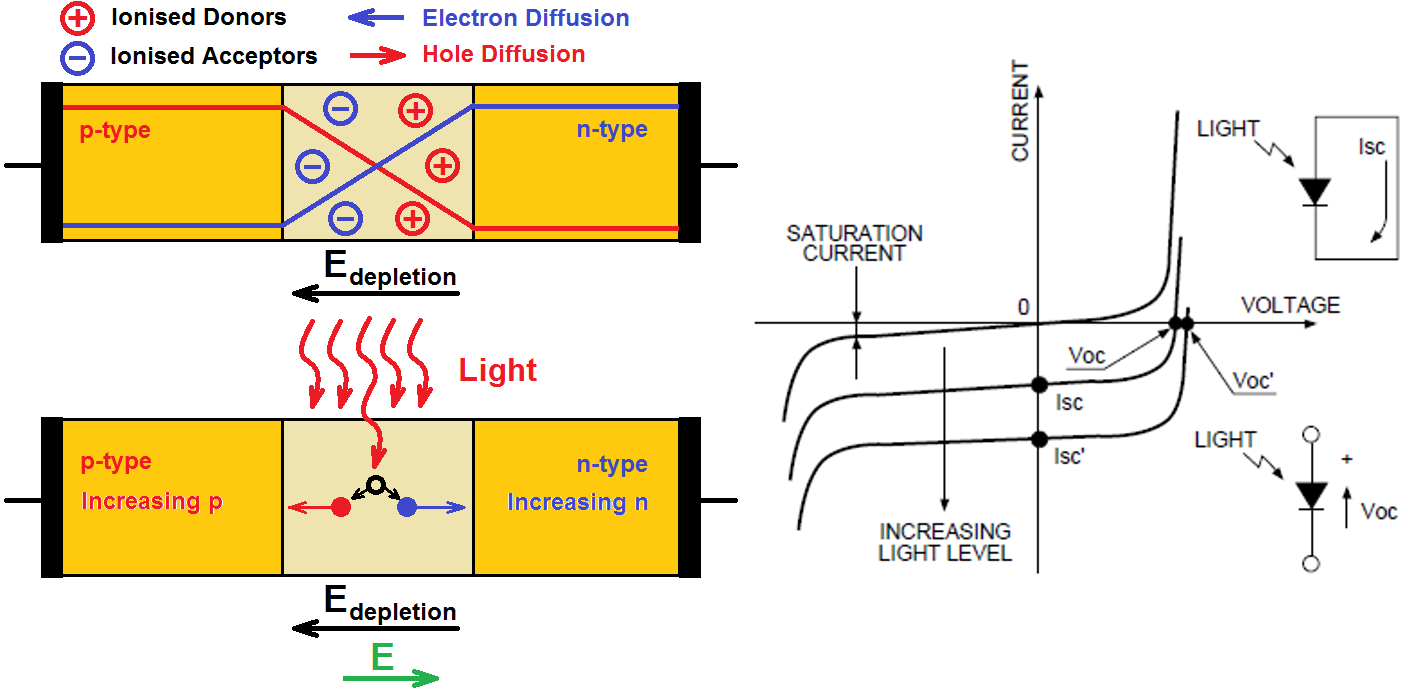
\includegraphics[scale=0.25]{obr02_char.png}
	\end{frame}
%------------------------------------------------------------------------------
	\begin{frame}
    \frametitle{Photodiode}
		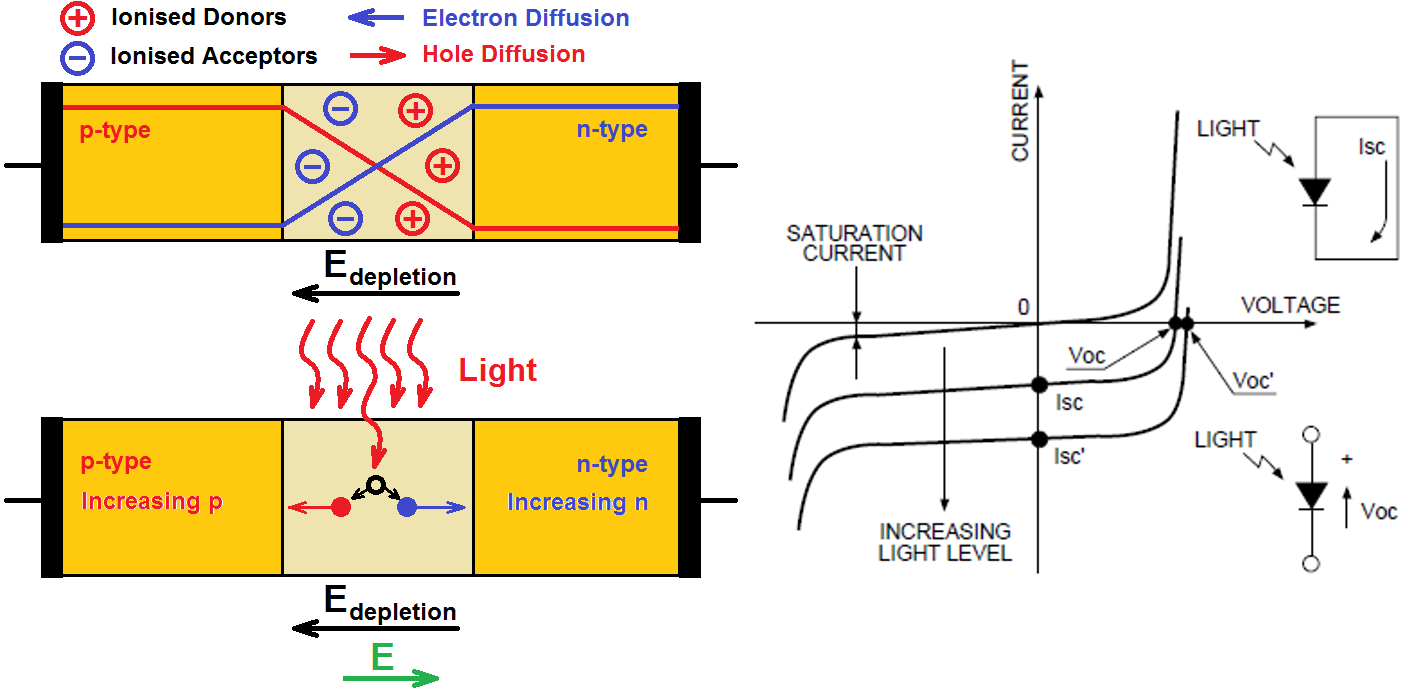
\includegraphics[scale=0.25]{obr02_char.png}\\
		Additional charge creates electric field that reduces the electric field of depletion area. Charge imbalance generates voltage across the terminals. The maximum open-circuit voltage corresponds to diode characteristic.
	\end{frame}
%------------------------------------------------------------------------------
	\begin{frame}
    \frametitle{Photodiode - Technology}
		\begin{center}
			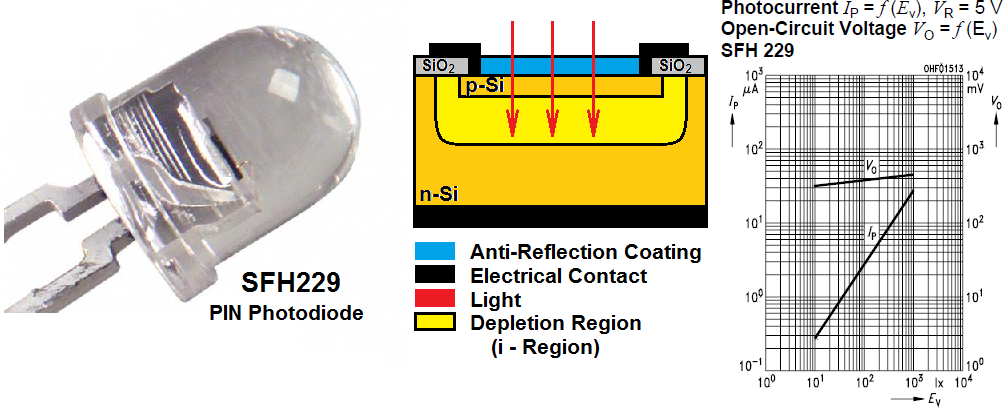
\includegraphics[scale=0.35]{obr01_fotodioda.png}
		\end{center}
		
		\begin{itemize}
			\item The PIN diode construction is often used to increase the size of depletion area.
			\item i-region is intrinsic or slightly doped area. Other parts are highly doped to get ohmic contact with leads.
		\end{itemize}
	\end{frame}
%------------------------------------------------------------------------------
	\begin{frame}
    \frametitle{VA Characteristic}
		\begin{tabular}{m{0.35\linewidth} m{0.5\linewidth}}
		\begin{center}
			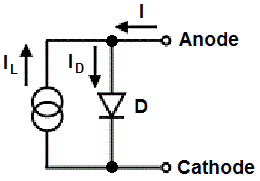
\includegraphics[scale=0.45]{obr12_nahrSch.png}
		\end{center}
		& \textbf{Modified Shockley Equation}
		$$I = I_D - I_L$$
		$$I = I_0\left(e^{\frac{U\cdot e}{n\cdot k\cdot T}}-1\right) - I_L$$
		\end{tabular}
		
		\begin{itemize}
			\item $I_L$ is the short-circuit current created by the incoming light.
			\item The equation above also defines temperature behavior of photodiodes and solar cells.
			\item The characteristic is also dependent on resistances of the leads (serial resistance should be included to the scheme).
		\end{itemize}
	\end{frame}
%------------------------------------------------------------------------------
	\begin{frame}
    \frametitle{Photo-Effect Efficiency}
		\begin{center}
			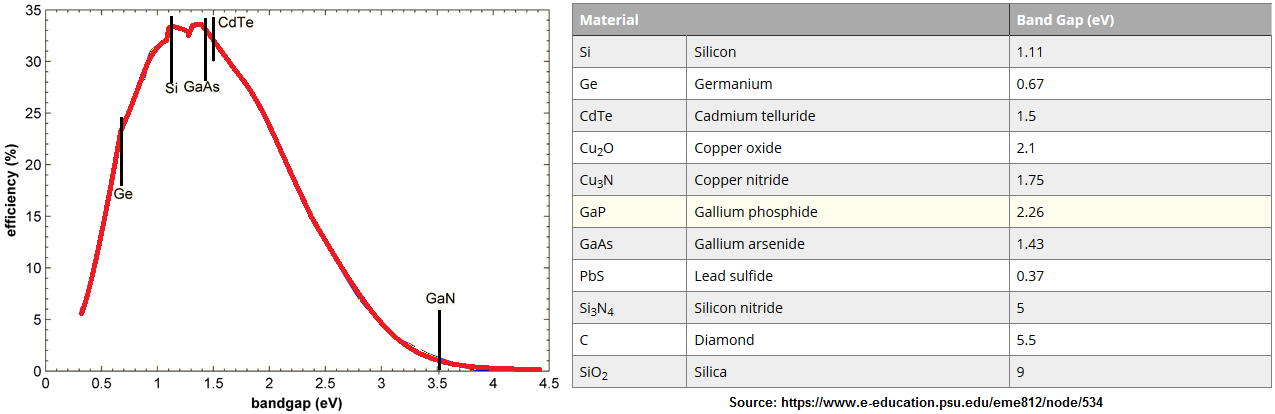
\includegraphics[scale=0.35]{obr03_ucinnost.png}
		\end{center}
		
		\begin{itemize}
			\item Energy higher than band gap energy is dissipated as heat.
			\item Most of the electrons are unable to cause photo-effect if the band-gap is to high.
		\end{itemize}
	\end{frame}
%------------------------------------------------------------------------------
%Photovoltaic
%------------------------------------------------------------------------------
\section{\texorpdfstring{Photovoltaic}{Photovoltaic}}
%------------------------------------------------------------------------------
	\begin{frame}
    \frametitle{Solar Cell}
		\begin{tabular}{m{0.38\linewidth} m{0.52\linewidth}}
		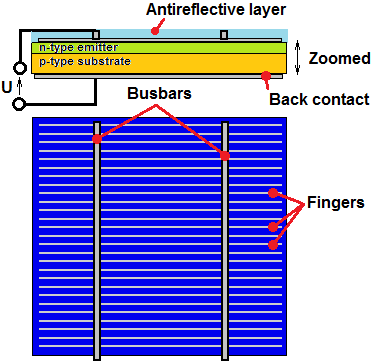
\includegraphics[scale=0.4]{obr06_konstrukce.png} &
		\small
		\begin{itemize}
			\item Solar cells increase the size of active photodiode area to get most of the power from incoming light.
			\item The contacts are made from silver printed on the semiconductor layer (screen printing).
		\end{itemize}
		\end{tabular}
		
		\begin{itemize}
			\item The Anode contact covers whole rear side of the cell.
			\item Bus bars are used to connect cells together in the panel.
			\item Reflective layer increased the light absorption.
		\end{itemize}
	\end{frame}
%------------------------------------------------------------------------------
	\begin{frame}
    \frametitle{Solar Cell - Materials}
		\begin{center}
			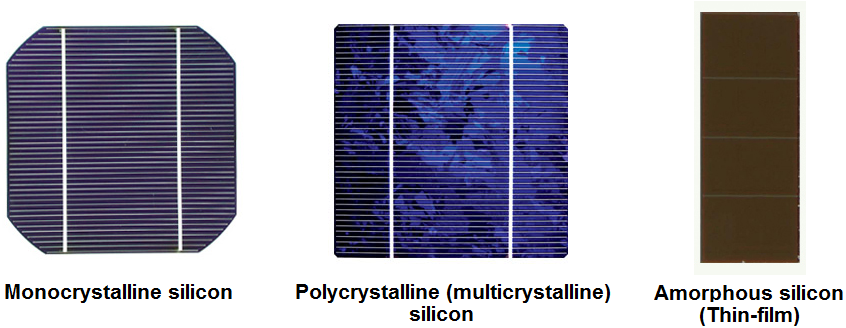
\includegraphics[scale=0.4]{obr05_druhy.png}
		\end{center}
		\textbf{Monocrystalline silicon}	
		\small
		\begin{itemize}
			\item oldest type, made from pure silicon crystal, iridescent blue or black color,
			\item[+] high efficiency - typical $\approx$15 \% (up to 22-24 \%), very durable,
			\item[-] efficiency gradually decreases (about 0.5 \% per year), brittle,
			\item[-] complicated manufacturing (from silicon slices), expensive. 
		\end{itemize}
	\end{frame}
%------------------------------------------------------------------------------
	\begin{frame}
    \frametitle{Solar Cell - Materials}
		\textbf{Polycrystalline silicon}	
		\small
		\begin{itemize}
			\item made by assembling grains and plates of silicon crystals, mosaic-like appearance,
			\item[+] good efficiency - typical $\approx$12 \%, very durable, cheaper technology - manufacturing smaller grains is less complicated,
			\item[-] less efficient than monocrystalline Si, brittle. 
		\end{itemize}
		\normalsize
		\textbf{Amorphous silicon}	
		\small
		\begin{itemize}
			\item deposition of silicon film onto substrate glass, dark colors (black, brown),
			\item[+] small amount of Silicon $\Rightarrow$ cheap, several substrates can be used for deposition $\Rightarrow$ flexible solar cell on plastic substrates,
			\item[+] less prone for overheating,
			\item[-] poor efficiency - typical $\approx$6 \%. 
		\end{itemize}
	\end{frame}
%------------------------------------------------------------------------------
	\begin{frame}
    \frametitle{Solar Cell - Materials}
		\begin{center}
			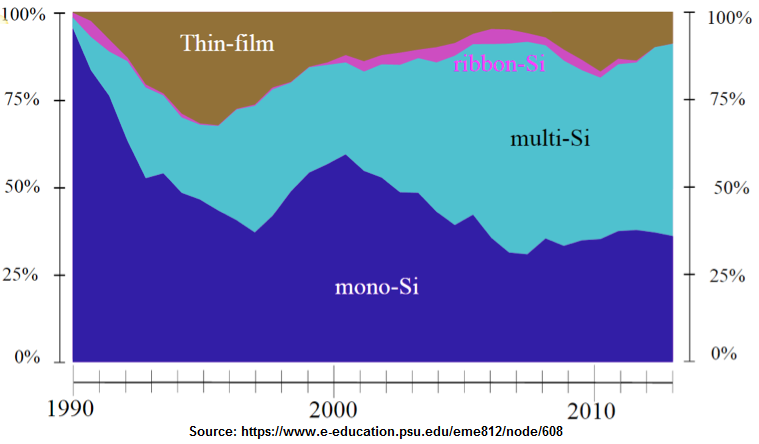
\includegraphics[scale=0.4]{obr04_vyvoj.png}
		\end{center}
		\textbf{Other thin film technologies}	
		\small
		\begin{itemize}
			\item Cadmium Telluride, CdTe: toxic Cd, high efficiency (16 \%).
			\item Copper Indium Gallium Selenide (CIGS): high efficiency (up to 19 \%), problematic deposition quality.
		\end{itemize}
	\end{frame}
%------------------------------------------------------------------------------
	\begin{frame}
    \frametitle{Equivalent circuit}
		\begin{center}
			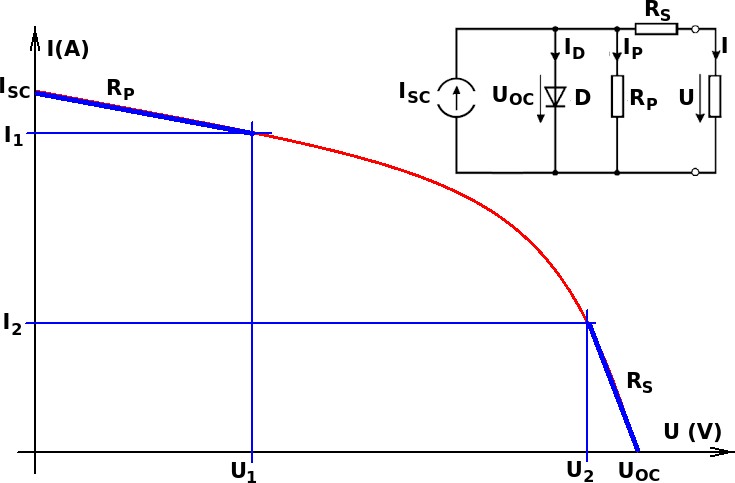
\includegraphics[scale=0.3]{obr07_odpory.png}
		\end{center}
		\small
		\begin{tabular}{m{0.45\linewidth} m{0.45\linewidth}}		
		\begin{itemize}
			\item[$U_{OC}$]... open-circuit voltage
			\item[$I_{SC}$]... short-circuit current
			\item[$R_{P}$]... shunt res., defects
			\item[$R_{S}$]... serial res., leads
		\end{itemize}
		& $$R_P=\frac{U_1}{I_{SC}-I_1}$$ $$R_S=\frac{U_{OC}-U_2}{I_2}$$
		\end{tabular}
	\end{frame}
%------------------------------------------------------------------------------
	\begin{frame}
    \frametitle{Power Got from the Solar Cell}
		\small
		\begin{tabular}{m{0.65\linewidth} m{0.25\linewidth}}
		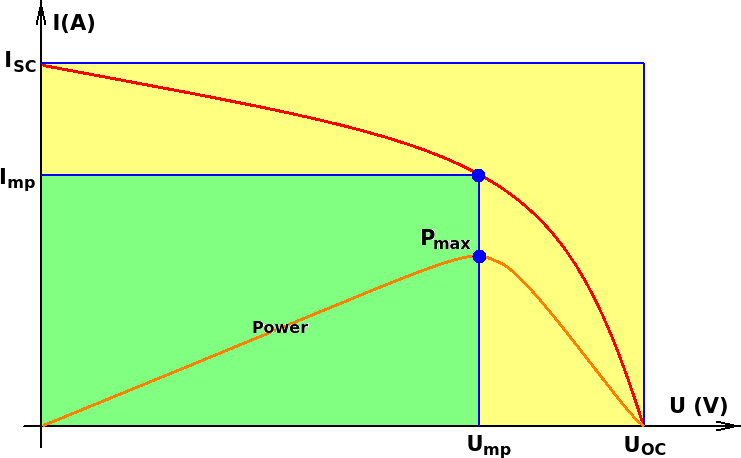
\includegraphics[scale=0.32]{obr08_plneni.png}
		\begin{flushleft}
			\textbf{Fill Factor}
		\end{flushleft}
		\small
		\begin{itemize}
			\item it defines the utilization of the solar cell,
			\item maximum varies with different materials,
			\item affected by $R_S$ and $R_P$ values!!!
		\end{itemize}
		& $$FF=\frac{U_{mp}\cdot I_{mp}}{U_{OC}\cdot I_{SC}}$$
		
		\textbf{Commercial}: $$FF\approx0.83-0.85$$
		\textbf{Efficiency}: $$\eta=\frac{U_{OC}\cdot I_{SC}\cdot FF}{P_{in}}$$
		
		\begin{itemize}
			\item[$P_{in}$]... incoming solar power
		\end{itemize}
		\end{tabular}
		
	\end{frame}
%------------------------------------------------------------------------------
	\begin{frame}
    \frametitle{Solar Panel}
		
		\begin{itemize}
			\item interconnected several solar cells together,
			\item serial connection increase the open-circuit voltage,
			\item parallel connection increase the short-circuit current.
			\item Interconnection of several panels creates solar arrays.
		\end{itemize}
		\begin{center}
			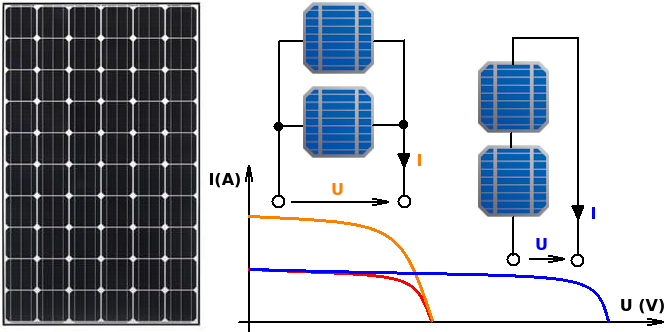
\includegraphics[scale=0.4]{obr09_panel.png}
		\end{center}
	\end{frame}
%------------------------------------------------------------------------------
\end{document}